\documentclass{sigchi-ext}
% Please be sure that you have the dependencies (i.e., additional
% LaTeX packages) to compile this example.
\usepackage[T1]{fontenc}
\usepackage{textcomp}
\usepackage[scaled=.92]{helvet} % for proper fonts
\usepackage{graphicx} % for EPS use the graphics package instead
\usepackage{balance}  % for useful for balancing the last columns
\usepackage{booktabs} % for pretty table rules
\usepackage{ccicons}  % for Creative Commons citation icons
\usepackage{ragged2e} % for tighter hyphenation
\usepackage{csquotes}

% Some optional stuff you might like/need.
% \usepackage{marginnote} 
% \usepackage[shortlabels]{enumitem}
% \usepackage{paralist}
% \usepackage[utf8]{inputenc} % for a UTF8 editor only

\copyrightinfo{}
%% EXAMPLE BEGIN -- HOW TO OVERRIDE THE DEFAULT COPYRIGHT STRIP --
% \copyrightinfo{Permission to make digital or hard copies of all or
% part of this work for personal or classroom use is granted without
% fee provided that copies are not made or distributed for profit or
% commercial advantage and that copies bear this notice and the full
% citation on the first page. Copyrights for components of this work
% owned by others than ACM must be honored. Abstracting with credit is
% permitted. To copy otherwise, or republish, to post on servers or to
% redistribute to lists, requires prior specific permission and/or a
% fee. Request permissions from permissions@acm.org.\\
% {\emph{CHI'14}}, April 26--May 1, 2014, Toronto, Canada. \\
% Copyright \copyright~2014 ACM ISBN/14/04...\$15.00. \\
% DOI string from ACM form confirmation}
%% EXAMPLE END

% Paper metadata (use plain text, for PDF inclusion and later
% re-using, if desired).  Use \emtpyauthor when submitting for review
% so you remain anonymous.
\def\plaintitle{Data Sculptures as a Playful and Low-Tech Introduction to Working with Data} \def\plainauthor{Rahul Bhargava, Caterine D'Ignazio}
\def\emptyauthor{}
\def\plainkeywords{data literacy; data physicalization; data sculptures; pedagogy; hands-on, case studies}
\def\plaingeneralterms{}

\title{Data Sculptures as a Playful and Low-Tech Introduction to Working with Data}

\numberofauthors{2}
% Notice how author names are alternately typesetted to appear ordered
% in 2-column format; i.e., the first 4 autors on the first column and
% the other 4 auhors on the second column. Actually, it's up to you to
% strictly adhere to this author notation.
\author{%
  \alignauthor{%
    \textbf{Rahul Bhargava}\\
    \affaddr{MIT Center for Civic Media} \\
    \affaddr{Cambridge, MA, USA} \\
    \email{rahulb@mit.edu} }
  \alignauthor{%
    \textbf{Catherine D'Ignazio}\\
    \affaddr{Emerson Engagement Game Lab}\\
    \affaddr{Boston, MA, USA}\\
    \email{catherine\textunderscore dignazio@emerson.edu} } }

% Make sure hyperref comes last of your loaded packages, to give it a
% fighting chance of not being over-written, since its job is to
% redefine many LaTeX commands.
\definecolor{linkColor}{RGB}{6,125,233}
\hypersetup{%
  pdftitle={\plaintitle},
%  pdfauthor={\plainauthor},
  pdfauthor={\emptyauthor},
  pdfkeywords={\plainkeywords},
  bookmarksnumbered,
  pdfstartview={FitH},
  colorlinks,
  citecolor=black,
  filecolor=black,
  linkcolor=black,
  urlcolor=linkColor,
  breaklinks=true,
}

% \reversemarginpar%

\begin{document}

\maketitle

% Uncomment to disable hyphenation (not recommended)
% https://twitter.com/anjirokhan/status/546046683331973120
\RaggedRight{} 

% Do not change the page size or page settings.
\begin{abstract}
There is a large and growing population of novice learners entering the field of working with data to tell stories, but they face many challenges related to process, methods and tools. This paper argues that activities focused on building physical manifestations of data, where some variable is mapped onto a physical artifact, are uniquely well-suited to scaffolding a process and exposing learners to methods so that they may take the next step in a learning journey.  We introduce our pedagogical motivations as well as three principles that guide our work - use familiar materials, stay low-tech, and create a playground.  Three case studies demonstrate how the playful activities we create based on these principles help novice learners explore advanced concepts very quickly.  This work strongly suggests that creating data sculptures helps novices overcome initial barriers to learning, set expectations for a data storytelling process, and feel empowered to take the next step.
\end{abstract}

\keywords{\plainkeywords}

\section{Introduction}
The surge in popularity of data visualization, fueled by "big data" narratives in popular press and viral infographics on social media has led large numbers of novices to enter the field of data-driven storytelling. These novices include students wanting to launch careers, nonprofit staff wanting to create change in new ways, journalists creating new forms of reporting, and engineers wishing to communicate complicated concepts clearly and effectively.

Unfortunately, the complexity and technological underpinnings of the data analysis pipeline are intimidating to newcomers. To understand these challenges better, we can look at survey responses about barriers to working with data collected by a local nonprofit training program\footnote{The surveys were conducted by our collaborator Tech Networks of Boston and TNB Labs at 5 unique sessions they hosted in early 2017 (n=340). A more thorough coding and analysis of these results is beyond the scope of this short paper.}. When asked "What are your biggest challenges?" when working with data, a lightweight analysis shows answers centered on themes related to technical complexity and a lack of awareness of both process and tools.  For instance, many pointed to a "lack of knowledge". Others mentioned "finding appropriate/right models/tools" or "Finding the right technology". Many came to the workshops to "get more experience" on "communication of impact".

These survey responses document the attitudes and anxieties that we have encountered in workshop settings with novices over the past ten years. The process of going from data to story is perceived as a dark art or a black box. While there are many learning materials online, these tool trainings\footnote{Tableau is just one of the many tool companies that provides an extensive set of video-based trainings: https://www.tableau.com/learn/training} and academic modules\footnote{Online learning modules for those wishing to enter the field of data science have taken off.  See this example on Udemy: https://www.udemy.com/datascience/} require a higher level of buy-in than most novice learners can afford.  They focus on technical language and digital technologies, two areas that intimidate novices that might not have digital fluency.

We argue that the activity of creating low-tech physicalizations of data is particularly well-suited to introduce novices to the process of finding stories in data and telling these stories to others. Specifically, producing three dimensional physical encodings of data quickly, with familiar materials, lets these learners enter the space of working with data in an unintimidating way. These learners want to tell stories with their data, not become "data analysts".  With this audience in mind, we refer to these objects by the much more friendly name of  "data sculptures"\footnote{It is hard to trace the original use of the term, but Bhargava was first exposed to it in 2013 via an episode of the Data Stories podcast \cite{Bertini_Stefaner}}.

Three principles guide the Data Sculpture activities that we believe carry these benefits:
\begin{itemize}
  \item \textbf{Use familiar materials}: This reduces the psychological barriers to learning; meeting learners where they are and building their confidence.
  \item \textbf{Go low-tech}: This allows for a focus on underlying concepts and mental models needed to work with data, regardless of the toolchain employed once the learner is further along in  their journey.
  \item \textbf{Create a playground}: Allowing the learner to move from data to story quickly, with acknowledged disregard for nuance and details, models the longer process and helps them build confidence for taking the next step.
\end{itemize}

This paper supports our argument with short case studies from 10 years of leading hands-on data sculpture activities in a variety of educational settings.  First, we discuss doing short 5-minute building activities in professional development workshops with non-expert audiences.  Second, we look at creations made by undergraduate and graduate students in week-long data sculpture "sketching" exercises.  Third, we look at some nascent work introducing data sculptures to elementary school students in classroom settings. We reflect on each of these settings to support our argument that data sculptures are a uniquely appropriate approach for helping novice audiences move past the barriers they see to building their data literacy.

\section{Pedagogical Inspirations}

Our engaged workshops draw inspiration from a number of existing pedagogical approaches. One central idea is Seymour Papert's Constructionist approach to learning. Papert argues that the most meaningful learning experiences come when learners are deeply engaged in designing and creating things \cite{Papert_1993}.  These physical objects we create embody our learnings, and serve as physical foils which others can react to and reflect on. The interactive dialog through and with these objects is a powerful path to learning. Another central idea, inspired by the history of feminist thinking, is to reframe who is allowed, and who isn't allowed, to create with data \cite{DIgnazio_Klein_2016}.  Data sculptures provide an opportunity to empower more diverse audiences to tell stories with data that can create change in the world around them. What follows is a brief background of the theory behind each of our three underlying principles. 

\subsection{Use Familiar Materials}

\begin{marginfigure}[-15pc]
  \begin{minipage}{\marginparwidth}
    \centering
    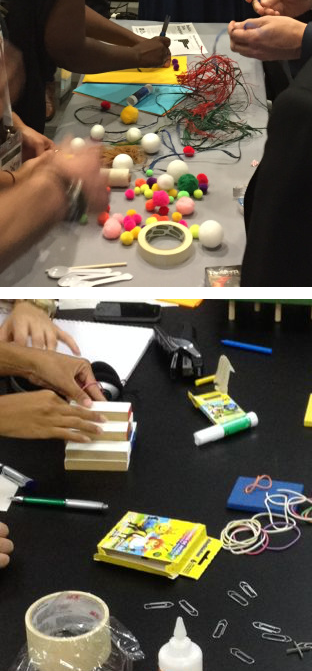
\includegraphics[width=1.0\marginparwidth]{figures/materials}
    \caption{Examples of some of the types of materials used to create quick data sculptures.}~\label{fig:materials}
  \end{minipage}
\end{marginfigure}

This principle harkens back to the founders of our current model of approaching pedagogy.  We can begin with Piaget's dismissal of the idea of learners as empty vessels to be filled with knowledge. He advocated for respecting learners' lived experiences and how those experiences either "assimilated" new knowledge, or had to be adapted to "accommodate" it \cite{Piaget_1952}. We also draw inspirations from Freire's approach to contextualizing content in the settings that matter to the learner \cite{Freire_1968}. For Freire, the material artifacts were a strong component of creating a connection between the learner and the content.  Another inspiration can be found in the work of James Rojas, who reinterprets urban planning as participatory play by using low-tech materials to engage the general public in discussions \cite{Rojas_Kamp_2016}. Our data sculpture activities use a variety of physical craft materials sourced from near the site of each workshop (see Figure~\ref{fig:materials}).

\subsection{Go Low-Tech}

It is critical to keep in mind novice learners when designing ways for newcomers to enter a technology-oriented space. There are numerous interesting high-tech physical interfaces being created, many of them emerging from the field of tangible interfaces \cite{Ishii_2008, Houben_2016, Taher_Hardy_2015}. We find more appropriate inspiration for our contexts in work such as "squishy circuits" \cite{Johnson_Thomas_2010}, "crafting technology" \cite{Buechley_Perner_2012}, and "data edibilization" \cite{Wang_Ma_Luo_Qu_2016}. These approaches present an opportunity to create something in a physical language that is familiar and delightful to the learner.  These echo the ideas of Froebel's gifts - which gave kindergarten children building blocks to construct with that made sense for their natural world and setting \cite{Fröbel_1885}. More recent work has found that in settings where one wants to promote interactive dialog with the audience about the data, informal presentations of data can work better than formal ones \cite{Bhargava_Kadouaki_Bhargava_Castro_DIgnazio_2016, Wood_Isenberg_Isenberg_Dykes_Boukhelifa_Slingsby_2012}. These approaches are driving a rethinking of civic and political action in democracies, towards more data-centric and visualized processes that might offer more opportunity for engagement \cite{Bohman_2015, Zhao_Moere_2008, Jansen_2015}.

\subsection{Create a Playground}

There is a long history of participatory workshops that inspire our approach. Recent work has brought this history to data physicalization \cite{Huron_Carpendale_Boy_Fekete_2016}.  In addition, we follow the guidance of noted developmental psychologist and learning researcher Edith Ackermann.  She reminds us why hands-on, arts-based workshops can be a powerful setting by noting that "in a playful environment you feel safe enough to explore ideas that would otherwise be risky" \cite{Ackermann_2014}. This guidance suggests a pathway to overcoming the fear felt by many novice learners, by carefully crafting the activity environment so they do feel "safe" - a key precondition to receptiveness to learning. However, Ackermann  also notes that "you cannot use play or fun as a pretext". The playful approach you craft must be deeply tied to the topic at hand; and must help learners take the next step in a learning journey.

\section{Case Studies}

With these pedagogical inspirations and guiding principles in mind, we can begin to discuss the settings we have created.  In each we will support our argument that creating low-tech physicalizations of data is uniquely well-suited to introduce novices to the process of finding stories in data and telling these stories to others.

\subsection{Data Sculptures as a Workshop Ice-Breaker Activity}

\begin{marginfigure}[-25pc]
  \begin{minipage}{\marginparwidth}
    \centering
    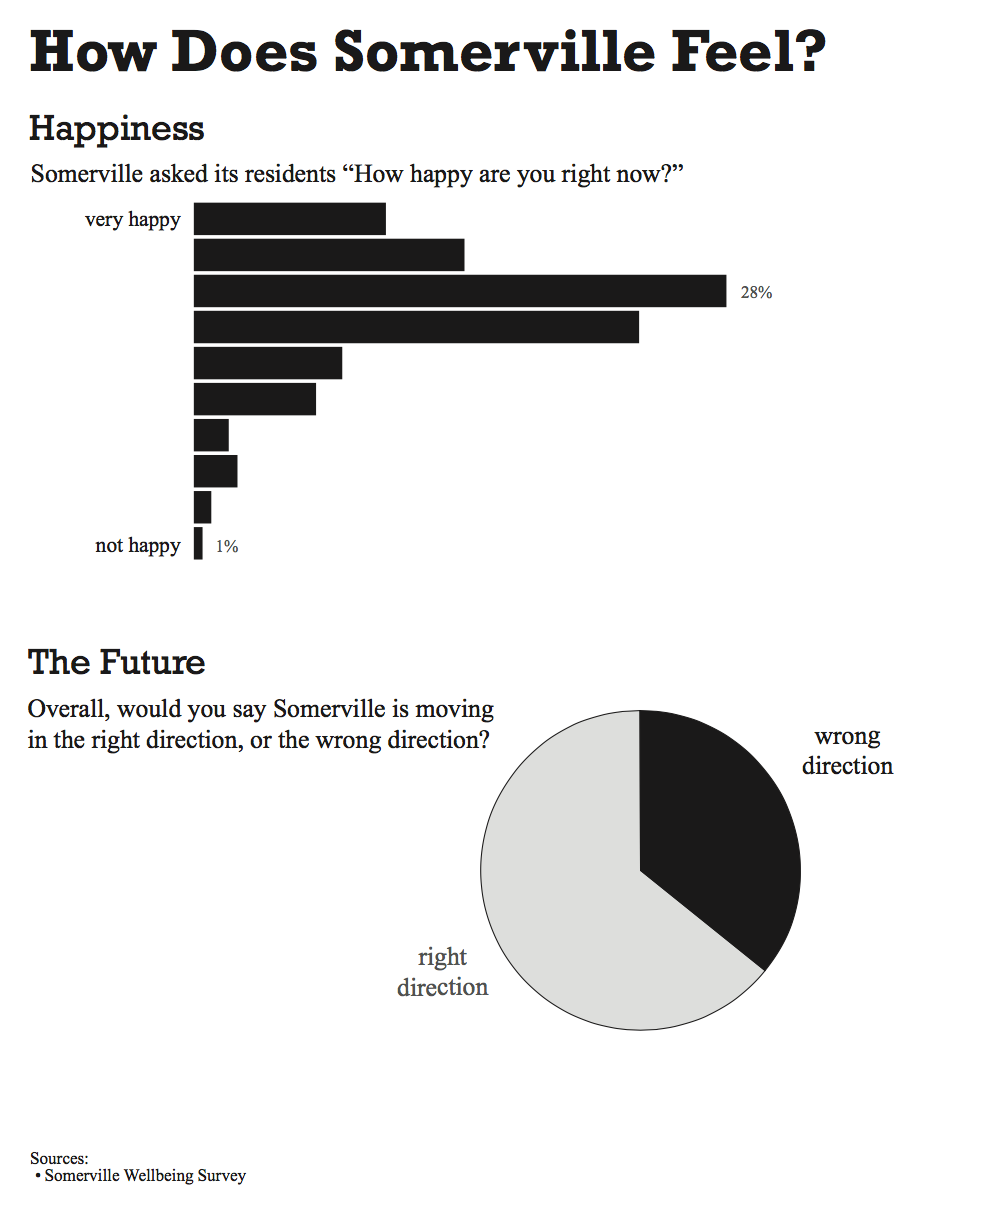
\includegraphics[width=1.0\marginparwidth]{figures/data-sculpture-handout}
    \caption{A sample of the type of one-page handout used to support the Data Sculpture activity in a workshop setting.}~\label{fig:handout}
  \end{minipage}
\end{marginfigure}

Professional development settings are fraught with failed attempts to build data literacy, or a data culture, within corporate walls.  These efforts, usually led by the IT department, generally involve tool trainings and long days in front of computer screens.  This seldom relates to the problems faced by ordinary staff, often instead attempting to train them in the emerging field of data science.


\begin{marginfigure}[-5pc]
  \begin{minipage}{\marginparwidth}
    \centering
    \includegraphics[width=1.0\marginparwidth]{figures/sculpture-examples}
    \caption{Two data sculptures created by participants at a workshop.}~\label{fig:mitsculptures}
  \end{minipage}
\end{marginfigure}

Over the last ten years we've run short data sculpture exercises at dozens of workshops targeting this audience.  Our short activity involves working with the key stakeholders before the workshop to develop a simple 1-page data handout, summarizing some relevant data with traditional charts and graphs (see Figure~\ref{fig:handout}).  Recent work on "Data Placemats" has explored the role of these types of handouts in building understanding when bringing together groups around data \cite{Pankaj_Emery_2016}.  Generally, during the workshop a central table holds materials carefully selected from local vendors, made with local materials.  Participants are then told to pair up and given 6 minutes to build something that represents some story in the data they see.  Key advice includes thinking with their hands, and not simply creating a bar chart out of pipe cleaners or other such materials.

A facilitated discussion after the frenzied building period allows opportunities for highlighting the depth of storytelling that can be done with such simple materials, on multiple axes.  There is inevitably a rich visual symbology developed.  There is always a variety of types of stories told (comparison stories, stories over time, "factoid" stories, etc).  Visual and physical variables can be explored by noting creative use of color, size and positioning (see Figure~\ref{fig:mitsculptures}). These questions of narrative structure, variable mapping, and symbology that the participants constructions raise relate to the current issues of study in the field of data visualization and physicalization \cite{Jansen_2015}.  Novice learners often struggle with going from data, to story, to visual presentation, yet in this activity they can experiment with all three in a simple, unintimidating setting with familiar materials.  We find that participants recognize the ease with which these underlying concepts transfer over to more complicated (digital) tools available, achieving a key learning outcome.

\subsection{Week-Long Higher Education Data Sculptures Sketches}

Over the last three years Bhargava has taught a "Data Storytelling Studio" course at the undergraduate and graduate levels at MIT (through the humanities department).  This attracts students from across institutions and disciplines with a hands-on exploration of the strengths and weaknesses of various techniques for telling data-driven stories.  These techniques include traditional charts and graphs, mapping, interactive games, data sculptures, and more.  Each technique is tackled by small groups with just one week to go from sample data to a "sketch" of an idea.  The data sculptures students make illustrate their ability to think about what kind of stories are well suited to be told with physical materials\footnote{Explore 2016 sketches at http://datastudio2016.datatherapy.org/}.

These students are generelly technically adept, so they focus on how to put a story together and tell it to a specific audience. An illustrative sketch from a student group in 2016 focused on refugee populations in the state of Massachusetts in the US.  Built on a flat map of the state, it included vertical bar charts to represent the population of refugees from different home countries in various major cities in the area (see Figure~\ref{fig:massrefugees}).  This allowed for a quick interpretation by viewers familiar with the state's geography, and basic visual data literacy.  However, each physical bar opened up and contained a stack of cards representing various members of that community, which they included to "quite literally gives a glimpse into the lives of refugee populations in MA" (student quote).

\begin{marginfigure}[-7pc]
  \begin{minipage}{\marginparwidth}
    \centering
    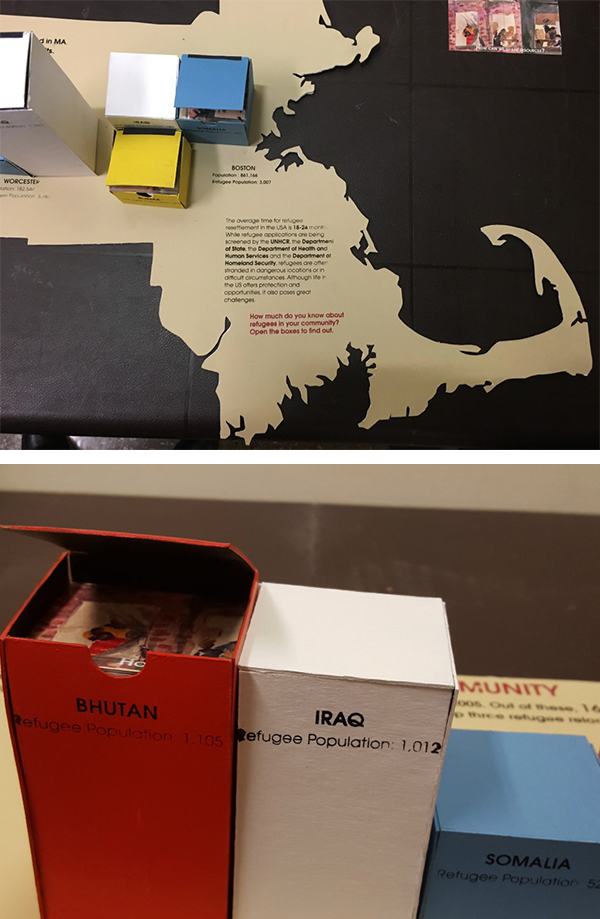
\includegraphics[width=1.0\marginparwidth]{figures/mass-refugees}
    \caption{A data sculpture about refugees in Massachusetts.}~\label{fig:massrefugees}
  \end{minipage}
\end{marginfigure}

This sketch, created by a team of 4 in just one week of in-class and out-of-class time, demonstrates fluency with a number of basic questions related to telling stories with data.  The sketch picks a subset of the data related to a story the learners care about. They write that they wanted to tell this story "because the integration challenges that refugee populations face is something that should involve the entire host community". The sketch maps data onto visual variables in multiply reinforced ways - "because it is very legible and because it resembles a building, an image that situates our project within the urban and/or social context of each city" (student writing).  It mixes quantitative and qualitative data. It builds on that mix to offer an invitation for readers to explore a deeper layer of reading to flesh out the significance of the data story - to perform a "physical action intending to reveal more information about refugee population in that city" (student writing).  This project demonstrates how in a short period of time the students were able to explore some fundamental concepts of creating data sculptures - the mapping of physical variables, allowing for layers of reading, and careful combination of elements to construct a physically interactive story.  They argue that this combination serves to "bring across our message for the need of integration of refugee and native communities and to show how we are already all living side-by-side" (student writing).

\subsection{Data Sculptures for Elementary School Students}

Elementary school programs around the world have recently joined the STEAM movement - including the Arts along with the Science, Technology, Engineering, and Math curricular focus \cite{Maeda_2012}. Data sculptures are well suited to this STEAM approach, leading us to explore opportunities with youth. Recently we've worked the MIT Museum and a network of primary schools around the globe to create a "creativity challenge" related to data.  After being introduced to data sculpture techniques at a training with Bhargava, teachers led K-5 students at 10 schools in identifying a topic to research, collecting data, and creating presentations to tell a data-driven story.  Working with this age group to build data literacy provides a unique set of challenges and opportunities related to vocabulary, visual literacy, and statistical literacy \cite{Hautea_Dasgupta_Hill_2017, Dasgupta_Hill_2017}.

This nascent collaboration suggests that thinking about the data as something that could be represented in physical form, both concretely and abstractly, is natural to these students.  One example is a group that investigated backpack weight across their school.  To convey the story of how heavy the average bag was back to their audience of peers, they filled a backpack with the correct weight of rocks "to see if people could hold it" (student participant). This literal mapping enhanced a poster board with more detailed data about their findings.  Another group at a different school creatively mapped air pollution to a more abstract artistic rendering on a loom (see Figure~\ref{fig:loom}).  In their own words, they:
\begin{displayquote}
...looked at the data by color coding the stripes.  They represent how the pollution was. So green is normal.  Yellow is more than normal.  Red is basically more than one hundred fifty.
\end{displayquote}

\begin{marginfigure}[-8pc]
  \begin{minipage}{\marginparwidth}
    \centering
    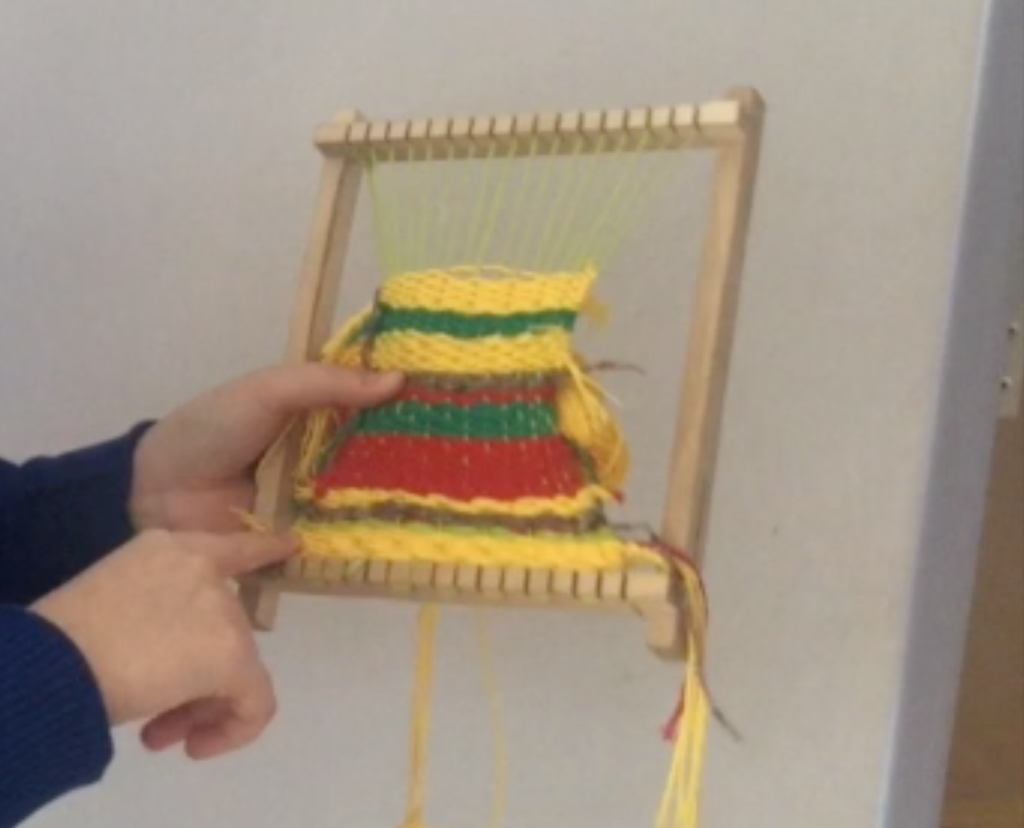
\includegraphics[width=1.0\marginparwidth]{figures/loom}
    \caption{An abstract representation of air quality in colors on a loom.}~\label{fig:loom}
  \end{minipage}
\end{marginfigure}

These examples, and others, suggest a strong willingness in young children to get excited about, and engaged in, data and physicalization on topics they care about.  These preliminary efforts point us towards future work to outline and document learning outcomes embodied by data sculptures in more detailed ways.  Piggybacking on the momentum and energy within the migration from STEM to STEAM could readily lead to a massive STEAM-powered rollout for data sculptures.

\section{Conclusion}

We argue that activity-based data sculptures with low-tech materials are uniquely suited to introduce novice learners into the field of working with data.  The examples above serve to back up the argument that novices in these settings can very quickly begin to engage problems that visualization experts face everyday, including selecting physical and visual variables, data mappings to those, layers of reading, and narrative structures.  Our pedagogical inspirations guide us to offer familiar materials that help these learners overcome any psychological barriers to entering the field and build self-efficacy.  The physical manifestation of a learner's data-driven story allows for reflective discussion and learning in lightweight collaborative learning communities.  This shifts the conversation around data from one between people and tools, to one between people and people, mediated by the physical artifacts they create.  This brings us back to approaches like Freire's, which thinks about learning and literacy as a path to empowerment rather than simply skill-building.  Our work strongly suggests that data sculptures are particularly well-suited to help novices overcome the barriers to learning and empower them to work with data to solve the problems they think are most important.

\balance{} 

\bibliographystyle{SIGCHI-Reference-Format}
\bibliography{sample}

\end{document}

%%% Local Variables:
%%% mode: latex
%%% TeX-master: t
%%% End:
